\chapter{Introduction of PitchApp}
\chapterauthor{by Boglarka Lehoczki}

\section{The Value PitchApp provides for Businesses}

PitchApp is intended to be a platform to help employees find the required organizational support to turn their ideas from inception to reality. The goal of our web application is, thus, to facilitate the launching of new projects. By making project ideas of colleagues easier and faster visible to management, PitchApp encourages employees to contribute more actively to the success of the company at which they work. In this way, PitchApp helps to achieve higher degrees of intrapreneurship, which leads to business growth. Using our application will bring companies ahead of the game, in terms of innovation and
employee engagement, as well as make big firms more competitive and flexible, thus more
profitable. Hence, “fast innovators take leadership positions in their industries” \parencite{SH90}.

\section{Characteristics of PitchApp}

PitchApp is a dynamic, single-page web application with database connection that we developed to enhance employee engagement and proactivity by connecting the employees’ ideas to even the highest levels of executives. Managers with budgets and resources for projects (i.e. potential future sponsors) can browse between different project ideas, which are posted by the employees. Distinct types of ideas are sorted into groups like HR, Procurement, R\&D etc., which facilitates searching among them. Then managers can offer their resources for the realization of a project idea, which they find valuable. Employees are also able to view the pitches posted by other colleagues in between their organization to avoid the sharing of redundant ideas. PitchApp is planned to be able to serve more large organizations at the same time and to be provided as a Software as a Service. PitchApp includes a user and session management system, which allows secure login and logout functionalities. It differentiates between public area, i.e. our landing page, and member area with two type of users, idea owners and idea sponsors.

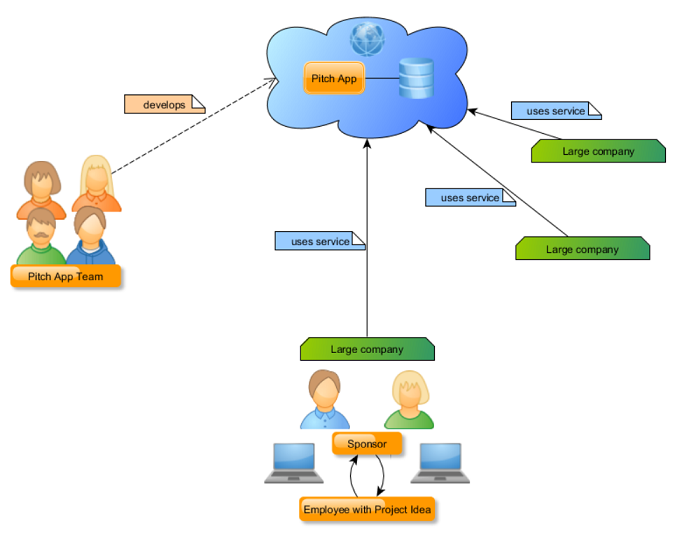
\includegraphics{pitchapp_saas.png}



\chapter{Architecture}
\chapterauthor{by Boglarka Lehoczki}

PitchApp is a web application and has a 3-tier architecture. The three tiers are the user interface, the application server and the database server. In such an architecture, the user interface runs in a web browser like Google Chrome or Mozilla Firefox. The user interface communicates with the application server through HTTP requests and responses, as the application server also implements web server functionalities. The application server itself acts as a client of the database server \parencite[p.~80]{MT17}. The interaction between these two servers can be based on different protocols or database connectivities, like JDBC for JAVA or ODBC for ABAP. The application server fetches the needed data from the database server, which returns it to the client in its reply. The process described above is shown by the following figure \parencite[p.~80]{MT17}.

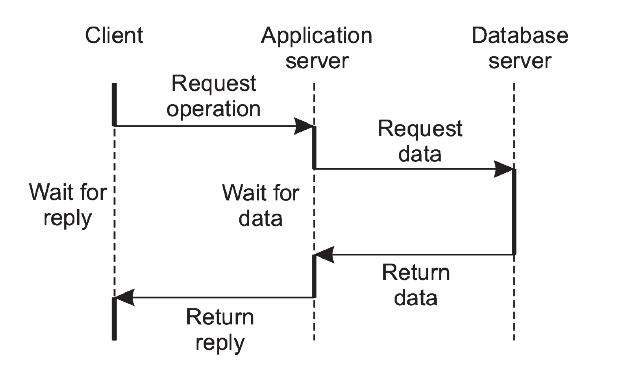
\includegraphics{3tiers_gen.png}

Developing a web application was a given requirement and it has several advantages. In comparison to a native application (with 2-tier architecture), the user do not have to install any additional application to its local machine, because the web application runs in a browser. From this also follows, that if in the future we e.g. change the user interface the user do not have to download updates onto his or her local machine. An other benefit of web applications is that they are easier to scale and the different tiers can be scaled separately based on the use case.  

\chapter{Technologies used for Implementation}
\section{React and Reactstrap}
\chapterauthor{by Boglarka Lehoczki}
\section{Okta}
\chapter{Final Results}
\chapter{User Manual}
\chapter{Difficulties of Implementation}
\chapter{Future Outlook: Missing Components and Functionalities}



